\documentclass[a4paper]{article}

%% Language and font encodings
\usepackage[english]{babel}
\usepackage[utf8x]{inputenc}
\usepackage[T1]{fontenc}

%% Sets page size and margins
\usepackage[a4paper,top=3cm,bottom=3cm,left=3cm,right=3cm,marginparwidth=1.75cm]{geometry}

%% Useful packages
\usepackage{amsmath}
\usepackage{graphicx}
\usepackage{url}
\usepackage[colorlinks=true, allcolors=blue]{hyperref}
\usepackage{amsfonts}
\usepackage{amsmath}
\usepackage{physics}
\usepackage{amssymb}
\usepackage{mathtools}

\numberwithin{equation}{subsection}
\newcommand{\mb}[1]{\mathbf{#1}}
\title{Magnetic propeties of a two dimentional electron gas strongly coupled to lights}
\author{K.Dini, O.V. Kibis and I.A. Shelykh}
\numberwithin{equation}{section}

\begin{document}

\maketitle

\section{Schrödinger problem for Landau levels in dressed 2DEG}

Our analysis is consider on 2 dimentional electronic gas which has distrubuted in $(x,y)$ plane in configuration space. We are going to examine the properties of 2DEG with stationary magnetic field
\begin{equation} \label{1.1}
  \vb{B} = (0,0,B)^T
\end{equation}
which directed on $z$ axis and a linearly $y$-polarized strong electomagnetic wave (dressing field) with electric field given by
\begin{equation} \label{1.2}
  \vb{E} = (0,E\sin(\omega t),0)^T
\end{equation}
which also propagate in $z$ direction. Here $B$ and $E$ represent the amplitude of the stationary magnetic field and electric field of dressing field.
\begin{figure}[ht!]
  \centering
  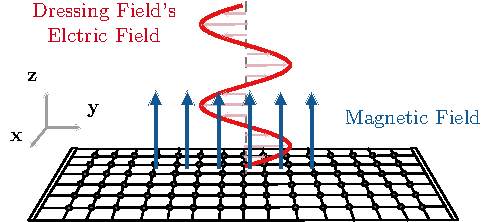
\includegraphics[scale=0.9]{figures/fig1.pdf}
  \caption{Stationary magnetic filed (blue color) and Strong EM wave (red color) applied to the 2DEG.}
  \label{fig:1.1}
\end{figure}

\noindent
Using Landau gauge for the stationary magnetic field we can represent it using vector potential as
\begin{equation} \label{1.3}
  \vb{A}_{s} = (-By,0,0)^T
\end{equation}
and choosing Coulomb gauge the dressing field can be present as the following vector potential
\begin{equation} \label{1.4}
  \vb{A}_{d}(t) = (0,[E/\omega ]\cos(\omega t),0)^T.
\end{equation}
Now the Hamiltonian of an electron in 2DEG can be reads as
\begin{equation} \label{1.5}
  \hat{H}_e(t) = \frac{1}{2m_e}\Big[\hat{\vb{p}} - e\big(\vb{A}_{s}+\vb{A}_{d}(t)\big)\Big]^2
\end{equation}
where $m_e$ is the effective mass of the electron and $e$ is the magnitude (without considering the sign of the charge) of the electron charge. This can be simplified to
\begin{equation} \label{1.6}
  \hat{H}_e(t) = \frac{1}{2m_e}\Big[
    (\hat{p}_x + eBy)\vb{e}_x +
    (\hat{p}_y - \frac{eE}{\omega}\cos(\omega t))\vb{e}_y
  \Big]^2
\end{equation}
where $\vb{e}_x$ and $\vb{e}_y$ are unit vectors along $x$ and $y$ directions respectively. Moreover,
\begin{equation} \label{1.7}
  \hat{H}_e(t) = \frac{1}{2m_e}\Big[
    (\hat{p}_x + eBy)^2 +
    (\hat{p}_y - \frac{eE}{\omega}\cos(\omega t))^2
  \Big]
\end{equation}
Since $[\hat{H}_e(t),\hat{p}_x] =0$ both operators share same eigenvalue and eigen functions which are free electron wave functions. Therefore we can modify the Hamiltonian as follows
\begin{equation} \label{1.8}
  \hat{H}_e(t) = \frac{1}{2m_e}\Big[
    ({p}_x + eBy)^2 +
    (\hat{p}_y - \frac{eE}{\omega}\cos(\omega t))^2
  \Big].
\end{equation}
Using momentum operator definition
\begin{equation} \label{1.9}
  \hat{p}_y = -i\hbar \pdv{y}
\end{equation}
we can modify Eq. \eqref{1.8} as
\begin{equation} \label{1.10}
  \begin{aligned}
    \hat{H}_e(t) & = \frac{1}{2m_e}\Big[
      ({p}_x + eBy)^2 +
      \Big(-i\hbar \pdv{y}- \frac{eE}{\omega}\cos(\omega t)\Big)^2
    \Big] \\
    & = \frac{1}{2m_e}\Big[
      ({p}_x + eBy)^2 +
      \Big(i\hbar \pdv{y} + \frac{eE}{\omega}\cos(\omega t)\Big)^2
    \Big].
  \end{aligned}
\end{equation}
Define the \textit{center of the cyclotron orbit} along $y$ axis as
\begin{equation} \label{1.11}
  y_0 \equiv \frac{-p_x}{eB}
\end{equation}
and the \textit{cyclotron frequency} as
\begin{equation} \label{1.12}
  \omega_0 \equiv \frac{eB}{m_e}.
\end{equation}
Then the Hamiltonian will leads to
\begin{equation} \label{1.13}
    \hat{H}_e(t) =
      \frac{m_e \omega_0^2}{2}(y-y_0)^2 +
      \frac{1}{2m_e}\Big(i\hbar \pdv{y}+\frac{eE}{\omega}\cos(\omega t)\Big)^2
\end{equation}
\begin{equation} \label{1.14}
  \begin{aligned}
    \hat{H}_e(t) =
      \frac{m_e \omega_0^2}{2}(y-y_0)^2 +
      \frac{1}{2m_e}\Big(
      -\hbar^2 \pdv[2]{y} & +
      i\hbar \pdv{y}\bigg[\frac{eE}{\omega}\cos(\omega t) \bigg] \\ & +
      \frac{i\hbar eE}{\omega}\cos(\omega t) \pdv{y}+
      \frac{e^2E^2}{\omega^2}\cos[2](\omega t)
      \Big)
  \end{aligned}
\end{equation}
\begin{equation} \label{1.15}
  \begin{aligned}
    \hat{H}_e(t) =
      \frac{m_e \omega_0^2}{2}(y-y_0)^2 +
      \frac{1}{2m_e}\Big(
      -\hbar^2 \pdv[2]{y} +
      \frac{2i\hbar eE}{\omega}\cos(\omega t) \pdv{y}+
      \frac{e^2E^2}{\omega^2}\cos[2](\omega t)
      \Big).
  \end{aligned}
\end{equation}
Let
\begin{equation} \label{1.16}
    (y - y_0) \rightarrow y
\end{equation}
and then this becomes
\begin{equation} \label{1.17}
  \begin{aligned}
    \hat{H}_e(t) =
      \frac{m_e \omega_0^2}{2}y^2 +
      \frac{1}{2m_e}\Big(
      -\hbar^2 \pdv[2]{y} +
      \frac{2i\hbar eE}{\omega}\cos(\omega t) \pdv{y}+
      \frac{e^2E^2}{\omega^2}\cos[2](\omega t)
      \Big).
  \end{aligned}
\end{equation}
Now assume that the solution for the time-dependent schrödinger equation
\begin{equation} \label{1.18}
    i \hbar \pdv{\psi}{t} = \hat{H}_e(t)\psi
\end{equation}
can be represent by the following form
\begin{equation} \label{1.19}
    \psi(\vb{r},t) = \frac{1}{\sqrt{L_x}} \exp\bigg(
      \frac{ip_x x}{\hbar} +
      \frac{ieE(y-y_0)}{\hbar \omega}\cos(\omega t)
    \bigg) \phi(y-y_0,t).
\end{equation}
Using the same subtution from Eq. \eqref{1.16} this becomes
\begin{equation} \label{1.20}
    \psi(x,y,t) = \frac{1}{\sqrt{L_x}} \exp\bigg(
      \frac{ip_x x}{\hbar} +
      \frac{ieEy}{\hbar \omega}\cos(\omega t)
    \bigg) \phi(y,t).
\end{equation}
Defining
\begin{equation} \label{1.21}
    \varphi(x,y,t) \equiv \frac{1}{\sqrt{L_x}} \exp\bigg(
      \frac{ip_x x}{\hbar} +
      \frac{ieEy}{\hbar \omega}\cos(\omega t)
    \bigg)
\end{equation}
we can simply the the Eq. \eqref{1.20} as
\begin{equation} \label{1.22}
    \psi(x,y,t) = \varphi(x,y,t) \phi(y,t).
\end{equation}
Let's subtitue Eq. \eqref{1.20} and Eq. \eqref{1.17} into Eq. \eqref{1.18} and we can observe that
\begin{equation} \label{1.23}
  \begin{aligned}
    \text{L.H.S} & = i \hbar \pdv{\psi}{t} =
    i \hbar \bigg( \pdv{\varphi}{t} \phi + \pdv{\phi}{t} \varphi \bigg) =
    i \hbar \bigg(
      \Big[\frac{-ieEy}{\hbar}\sin(\omega t)\Big]\varphi\phi +
      \varphi  \pdv{\phi}{t}
    \bigg) \\
    & =
    \big[{eEy}\sin(\omega t)\big]\varphi\phi +
    i \hbar\varphi  \pdv{\phi}{t}
  \end{aligned}
\end{equation}
and
\begin{equation} \label{1.24}
  \begin{aligned}
    \text{R.H.S} & = \hat{H}_e(t)\psi \\
    & =
    \bigg[
    \frac{m_e \omega_0^2}{2}y^2 +
    \frac{1}{2m_e}\Big(
    -\hbar^2 \pdv[2]{y} +
    \frac{2i\hbar eE}{\omega}\cos(\omega t) \pdv{y}+
    \frac{e^2E^2}{\omega^2}\cos[2](\omega t)
    \Big) \bigg]
    \varphi\phi
  \end{aligned}
\end{equation}
where we will can calculate this part by part as follows:
\begin{equation} \label{1.25}
  \begin{aligned}
    \frac{-\hbar^2}{2m_e}\pdv[2]{y}(\varphi\phi) & =
    \frac{-\hbar^2}{2m_e} \pdv{y}\bigg[
      \Big(\frac{ieE}{\hbar \omega} \cos(\omega)t\Big)\varphi\phi +
      \varphi\pdv{\phi}{y}
    \bigg] \\
    & =
    \frac{-\hbar^2}{2m_e} \bigg[
      \Big(\frac{ieE}{\hbar \omega} \cos(\omega)t\Big)^2\varphi\phi +
      \Big(\frac{ieE}{\hbar \omega} \cos(\omega)t\Big)\varphi\pdv{\phi}{y} +
      \Big(\frac{ieE}{\hbar \omega} \cos(\omega)t\Big)\varphi\pdv{\phi}{y} +
      \varphi\pdv[2]{\phi}{y}
    \bigg] \\
    & =
    \Big(\frac{e^2E^2}{ 2m_e\omega^2} \cos[2](\omega)t\Big)\varphi\phi -
    \Big(\frac{ieE \hbar}{m_e\omega} \cos(\omega)t\Big)\varphi\pdv{\phi}{y} -
    \frac{\hbar^2}{2m_e}
    \varphi\pdv[2]{\phi}{y}
  \end{aligned}
\end{equation}
and
\begin{equation} \label{1.26}
  \begin{aligned}
    \frac{2i\hbar eE}{2m_e\omega}\cos(\omega t) \pdv{y} (\varphi\phi)& =
    \frac{i\hbar eE}{m_e\omega}\cos(\omega t)
    \bigg[
      \Big(\frac{ieE}{\hbar \omega} \cos(\omega)t\Big)\varphi\phi +
      \varphi\pdv{\phi}{y}
    \bigg] \\
    & =
    \Big(\frac{-e^2E^2}{m_e\omega^2} \cos(\omega)t\Big)\varphi\phi +
    \frac{i\hbar eE}{m_e\omega}\cos(\omega t)\varphi\pdv{\phi}{y}.
  \end{aligned}
\end{equation}
Therefore we can derive that
\begin{equation} \label{1.27}
  \begin{aligned}
    \text{R.H.S} =
    \bigg[
    \frac{m_e \omega_0^2}{2}y^2
    -
    \frac{\hbar^2}{2m_e}
    \varphi\pdv[2]{\phi}{y} \bigg]
    \varphi\phi.
  \end{aligned}
\end{equation}
To satisfy the condition L.H.S$=$R.H.S we need to find a function $\phi(y,t)$ such that
\begin{equation} \label{1.28}
  \begin{aligned}
    \big[{eEy}\sin(\omega t)\big]\varphi\phi +
    i \hbar\varphi  \pdv{\phi}{t}
    =
    \bigg[
    \frac{m_e \omega_0^2}{2}y^2
    -
    \frac{\hbar^2}{2m_e}
    \varphi\pdv[2]{\phi}{y} \bigg]
    \varphi\phi
  \end{aligned}
\end{equation}
which can be simplyfied as
\begin{equation} \label{1.29}
  \begin{aligned}
    \bigg[
    \frac{m_e \omega_0^2}{2}y^2
    - {eEy}\sin(\omega t)
    -
    \frac{\hbar^2}{2m_e}
    \pdv[2]{y}
    - i \hbar \pdv{t}
    \bigg]
    \phi(y,t) = 0
  \end{aligned}
\end{equation}


























\end{document}
